\clearpage
\section{Diffusion coefficient}

The diffusion coefficient can be calculated with the Arrhenius relation:

\begin{align}
    \label{eq:1}
    D&=D_0 exp\left(-\dfrac{\Delta H}{RT}\right),
\end{align}
where $D$ is the Diffusion coefficient, $D_0$ is a pre-exponential factor, $\Delta H$ is the activation entalphy of diffusion in $J/mol$ (which is also represented as $Q$), R is the ideal gas constant ($8,314$ $J/K\cdot mol$) and $T$ is the temperature in Kelvin \citep{diff}. 

The linearization of Arrhenius relation can be made by taking the logarithm on both sides of equation \eqref{eq:1}, which yields:
\begin{align}
  \label{eq:2}
  ln(D)&=-\dfrac{\Delta H}{R}\dfrac{1}{T} + ln(D_0),
\end{align}
which is a linear equation where the slope is given by $-\Delta H/R$ and the intercept in the y-axis is given by $ln(D_0)$.

Considering that all systems have different temperature ranges, to proceed with the calculations, a new temperature range was chosen, from $450$ to $1950$ K, so that all systems use the same temperature range and can be compared with each other. The new temperature range was used to calculate $D$ for all systems, with a sample of 100 points evenly spaced, and the parameters of $D_0$, $Q$ and $R$ using equation \eqref{eq:1}.

After calculating the diffusion coefficient for the systems, the lorgarithm of the diffusion coefficients and the inverse of the temperature were also calculateded, in order to present the results in the linearized form of equation \eqref{eq:3}.

\subsection{Self diffusion}

The self-diffusing systems are Ag-Ag, Al-Al, Cu-Cu and Ti-Ti. Figure \ref{fig:self_diffusion} presents the graphs of the diffusion coefficient for the self-diffusion systems, where \ref{fig:self_d} shows the diffusion coefficient as a function of time and \ref{fig:self_lnd} shows the logarithm of the diffusion coefficient.

Figure \ref{fig:self_d} shows that the diffusion coefficient increases with the temperature, for all self-diffusion systems. It can also be noted from this plot, that the increase of the diffusion coefficient is higher for aluminum, than it is for the other systems, which indicates that there is faster self-diffusion for aluminum.

Figure \ref{fig:self_lnd} presents the logarithm of the self-diffusion coefficient as a function of the inverse of temperature, where the straight lines correspond to the linear behaviour expected from equation \ref{eq:2}. The plot shows that the titanium system has a steeper slope, which corresponds to a higher activation energy, meaning that it requires more energy for the diffusion to occur. On the other hand, the aluminum system has the less steep slope, which indicates a lower activation energy, requiring less energy for the diffusion to occur.

\begin{figure}[h]
 \centering
 %\captionsetup{justification=centering}
  \subfloat[]{
   \label{fig:self_d}
    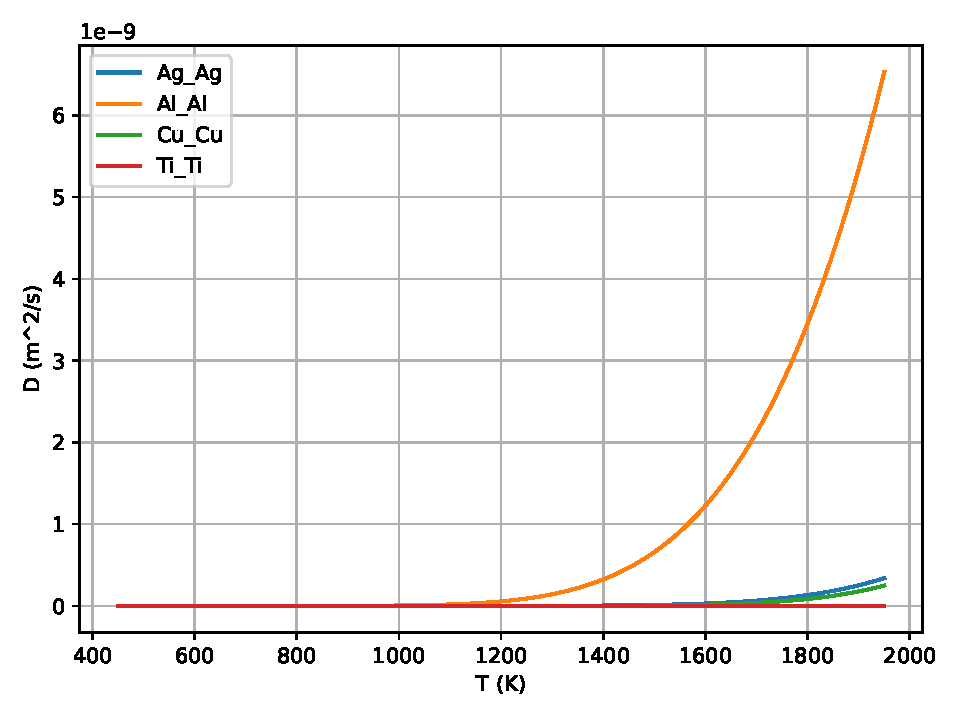
\includegraphics[width=0.5\textwidth]{graficas/D(T)_self.pdf}}
  \subfloat[]{
   \label{fig:self_lnd}
    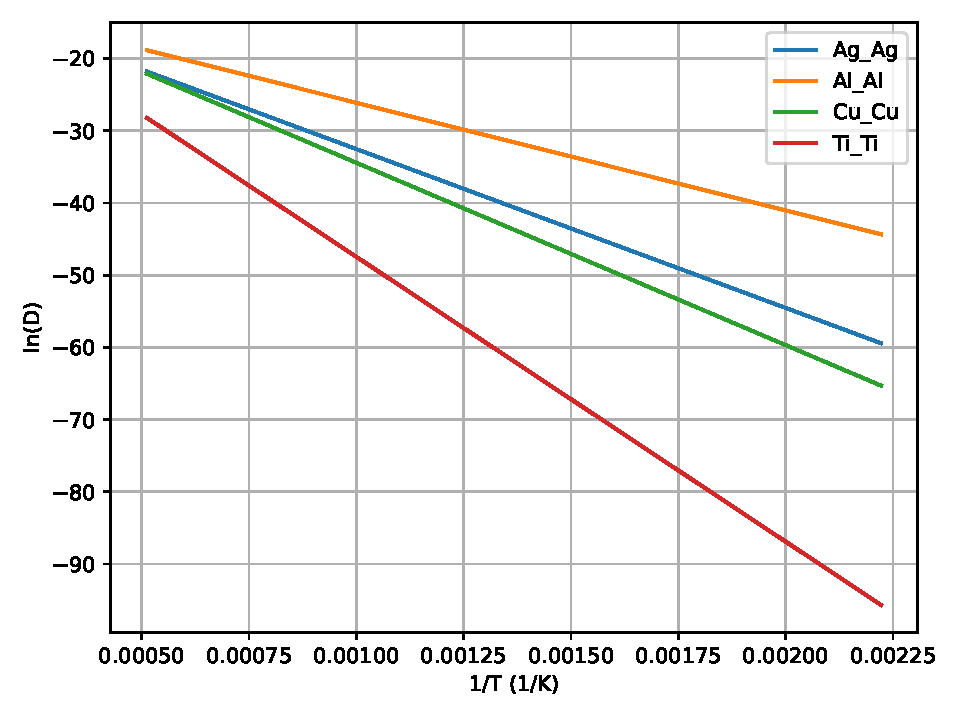
\includegraphics[width=0.5\textwidth]{graficas/ln(D)_self.pdf}}
 \caption{a) Diffusion coefficient $D$ ($m^2/s)$ as a function of temperature $T$ (K) and b) logarithm of the diffusion coefficient $ln(D)$ as a function of the inverse of the temperature $1/T$ ($K^{-1}$) for self-diffusion systems. \\
 \textit{Source: Data from \citep{kakusan}, visualization by the author (code available at \citep{mygit}).}}
 \label{fig:self_diffusion}
\end{figure}

\subsection{Solute diffusion}

The plot for the diffusion systems with aluminum and silver as solutes in copper, platinum and titanium are shown in figure \ref{fig:diffusion}.

Figure \ref{fig:d} presents the diffusion coefficient as a funciton of the temperature for all systems. It shows that for the system of Al-Cu (aluminum as a solute in copper) the diffusion coefficient increase is higher than for the other systems, indicating that aluminum can diffuse easier in copper.

Figure \ref{fig:lnd} shows the logarithm of the diffusion coefficient as a function of the inverse of the temperature. The plot presents straight lines that correspond to the beharivour expected from Arrhenius relation (equation \ref{eq:2}). 

For silver as solute, figure \ref{fig:lnd} shows that the system Ag-Ti has a steeper slope that the other two systems (Ag-Cu and Ag-Pt), this indicates that the activation energy for the Ag-Ti system is lower that it is for the other two systems, meaning that silver requieres more energy to diffuse in titanium that to diffuse on copper and platinum. It can also be seen that the system Ag-Cu has the less steep slope, which means a lower activation energy, indicating that silver requires less energy to diffuse in copper than in platinum and titanium. It can also be seen that both lines for Ag-Pt and Ag-Ti are close to each other, which corresponds to close values of activation energy.

In the case of aluminum as solute, in figure \ref{fig:lnd} it can be seen that the system Al-Cu has the less steep slope, corresponding to a lower activation energy. Meanwhile, the system Al-Ti has the steeper slope of these systems, which indicates that more energy is required for aluminum to diffue in tintanium than what it is required for it to diffuse in copper and platinum.

Overall, the Al-Ti system has a more steep slope than the other systems, indicating tha this system requires a higher energy for diffusion to occur. On the other hand, the system Ag-Cu presents the less steep slope, which indicates a lower activation energy, meaning that less energy is required for diffusion to occur in this system.

\begin{figure}[h]
 \centering
 %\captionsetup{justification=centering}
  \subfloat[]{
   \label{fig:d}
    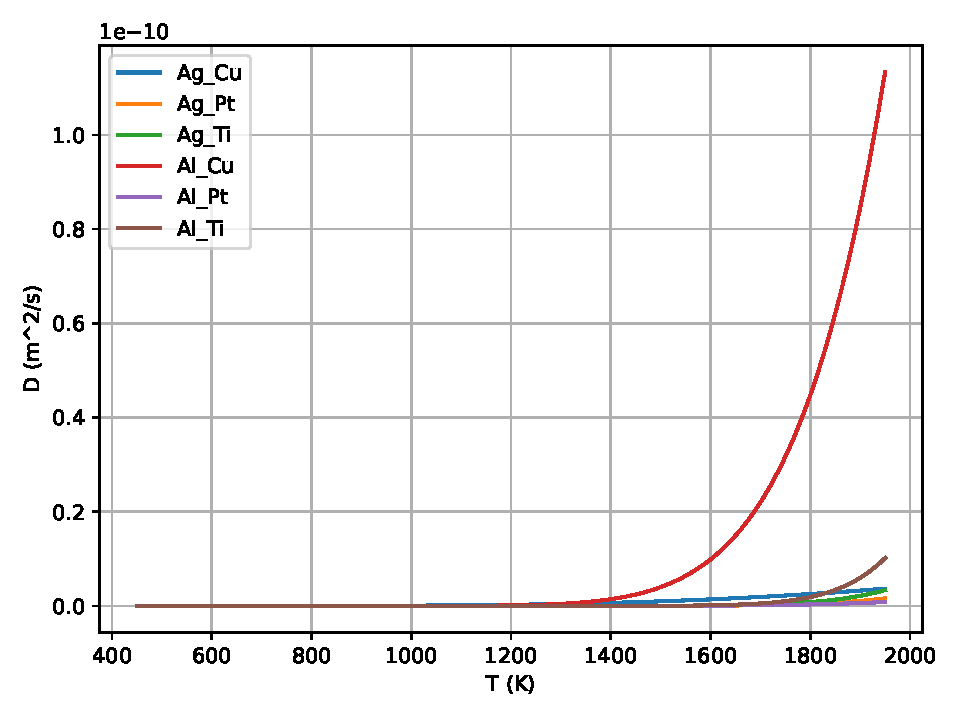
\includegraphics[width=0.5\textwidth]{graficas/D(T)_other.pdf}}
  \subfloat[]{
   \label{fig:lnd}
    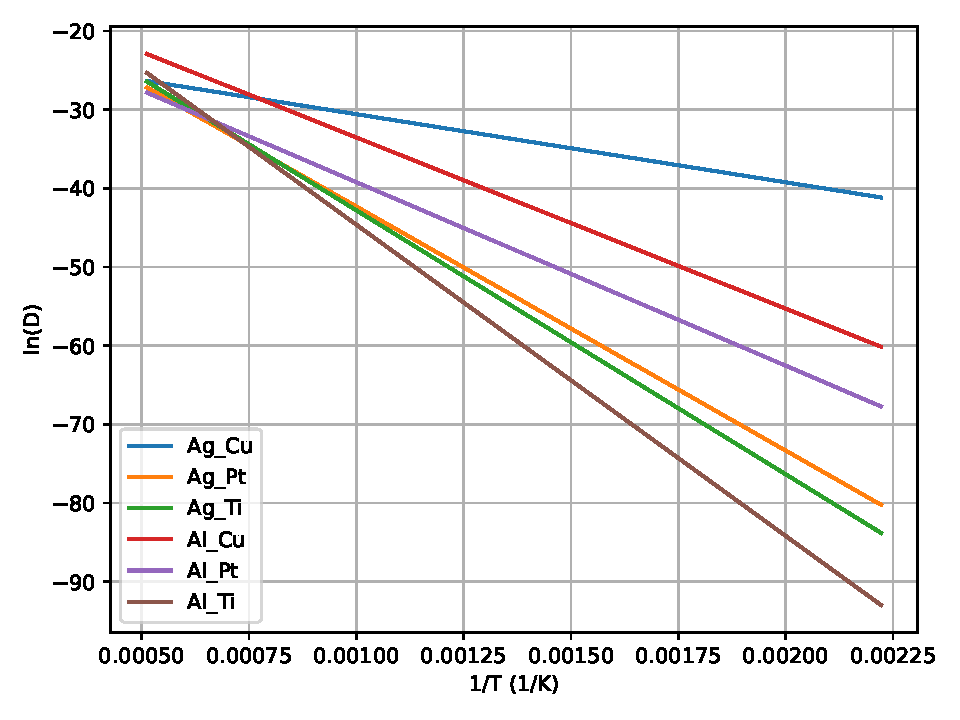
\includegraphics[width=0.5\textwidth]{graficas/ln(D)_other.pdf}}
 \caption{a) Diffusion coefficient $D$ ($m^2/s)$ as a function of temperature $T$ (K) and b) logarithm of the diffusion coefficient $ln(D)$ as a function of the inverse of temperature $1/T$ ($K^{-1}$). \\
 \textit{Source: Data from \citep{kakusan}, visualization by the author (code available at \citep{mygit}).}}
 \label{fig:diffusion}
\end{figure}